%!TEX root = ../dissertation.tex

\chapter{Architecture}
\label{chp:models}


\section{Composantes}

Dans cette section, nous faisons une présentation détaillée des composantes de notre STI. Il s'agit des composantes de base d'un STI tels que décrits dans le Chapitre\ref{chp:etat_art} : les modules tuteur, expert, apprenant et l'interface utilisateur.




    \subsection{Modèle Apprenant}   
 Le modèle de l'apprenant permet de décrire et de suivre la trace de l'évolution de l'apprentissage de l'apprenant, son niveau, ses lacunes, ses idées fausses, etc. Les données du modèle de l'apprenant sont mises à jour à partir des informations obtenues suite à ses décisions et ses actions au cours d'un partie.
 
  Dans SARAH, le modèle de l'apprenant sera, à terme, constitué des composantes suivantes :
 
\begin{enumerate}
\item  \textbf{Le Modèle Statique}, contenant des données statiques sur l'apprenant (nom, âge, type d 'apprenant,niveau scolaire, spécialité,  etc.).
\item  \textbf{Le Modèle cognitif} :  cette partie contient des informations sur l'état des connaissances de l'étudiant par rapport i la matière considérés (par exemple, les problèmes qu'il a résolus,
ses solutions, son niveau maîtrisé de la connaissances, etc..).\\\

Nous avons choisi le modèle de recouvrement ( Overlay) ( Carr et Goldstein, 1977) pour la représentation des connaissances de l'apprenant dans notre système. Dans ce modèle, les connaissances de l'apprenant sont construites sur les éléments de connaissance de l'expert (ou éléments de connaissance du domaine considéré) . Dans cette approche, les compétences indiquent clairement l'habileté de l'apprenant à utiliser ses connaissances. Cette méthode s'est avérée être un choix judicieux et adapté au contexte, car toutes les compétences à acquérir sont définies de manière intrinsèque et sans ambiguïté par les connaissances du domaine. La figure 3.2 présente le modèle Overlay. 

\begin{figure}
    \centering
    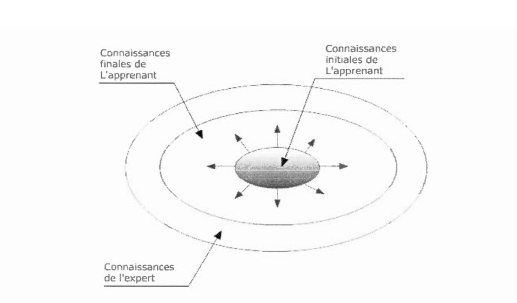
\includegraphics[width=0.75\textwidth]{figures/con1.PNG}
    \captionsetup{justification=centering}
    \caption{Représentation des connaissances de l'apprenant (modèle overlay)}
 \label{fig:2}
\end{figure}
\\\

\item  \textbf{Le Modèle des compétences}, contenant les croyances du système sur les compétences de l'apprenant. 
\item \textbf{Le Modèle Psychométrique}, contenant les informations permettant d'initialiser le modèle de l'apprenant en début de partie.
\item \textbf{Le Modèle Psychologique}, contenant les informations permettant de décrire les comportements et les processus mentaux de l'apprenant au fil des parties de jeu. 
\item \textbf{Le Modèle Affectif},ce modèle est un ensemble de données permettant de cerner les caractéristiques et les différentes facettes d'un étudiant. Il contient des connaissances relatives aux caractéristiques particulières permanentes ou momentanées de l'apprenant.
\item \textbf{Modèle d'inférences}: Pour nous, ce modèle contient les informations sur les modes d'inférences que l'apprenant applique dans son raisonnement (par exemple les modes inductif ou déductive que l'étudiant utilise dans ses résolutions de problèmes) [Shiri, 1997].
\item \textbf{Modeleur} : Le Modeleur a pour objectif de mettre à jour les connaissances de l'apprenant (gestion du modèle de l'apprenant); reconnaître ses bonnes performances; relever les connaissances erronées et suggérer des corrections. La Figure 3.2 illustre l'architecture du modèle de l'apprenant. Dans cette figure la notion « le comportement de l'apprenant )) inclue ses réponses aux questions. ses actions (comme la tâche d'adaptation). et les résultats de ces actions comme les solutions obtenues, etc.
\end{enumerate}
\begin{figure}
    \centering
    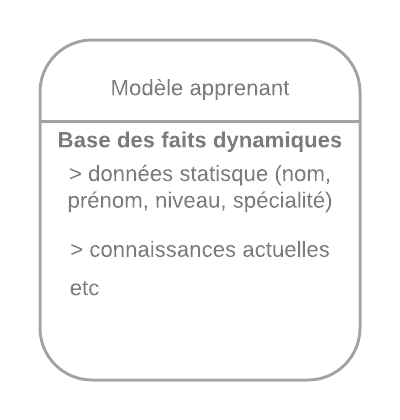
\includegraphics[width=0.75\textwidth]{figures/mod_app.png}
    \captionsetup{justification=centering}
    \caption{ Modèle de l'apprenant }
 \label{fig:m_app}
\end{figure}
\begin{figure}
    \centering
    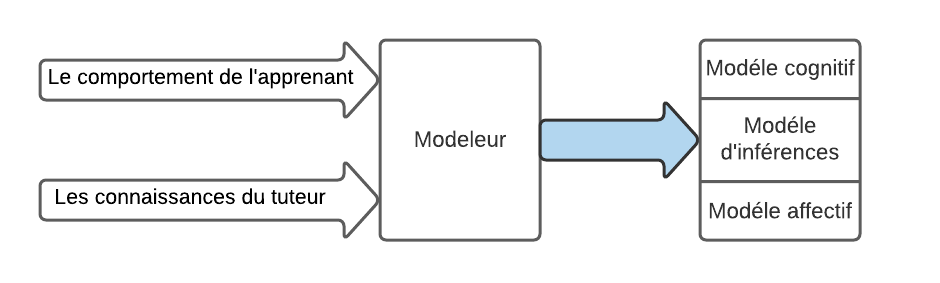
\includegraphics[width=0.75\textwidth]{figures/md_inf.png}
    \captionsetup{justification=centering}
    \caption{ L'architecture du modèle de l'apprenant }
 \label{fig:2}
\end{figure}
\\\


\subsubsection{Caractéristiques d'un sous-système modèle de l'apprenant }
Nous pensons que le sous-système modeleur est celui qui contient au moins les
caractéristiques suivantes :

\begin{enumerate}
\item la capacité de reconnaître les bonnes performances de l'apprenant (par exemple son niveau maîtrisé de la connaissance);
\item la capacité de relever les connaissances erronées;
\item la capacité de les expliquer (par exemple, informer l'apprenant s'il a choisi un cas inadéquat pour la résolution du problème donné. etc.);
\item  la capacité de suggérer des corrections (par exemple montrer les relations entre le problème courant et les problèmes similaires que l'apprenant a déjà résolus, etc.);
\item La capacité de mettre à jour les connaissances de l'apprenant; il doit être capable de  : \begin{itemize}
\item fixer l'ensemble des étapes à maîtriser par l'apprenant (par exemple; déterminer
tous les problèmes résolus);
\item découvrir les étapes maîtrisées mais non exprimées par l'apprenant (par exemple, découvrir les relations entre un problème résolu et le cas qu'il r choisi à cette fin);
\item découvrir les étapes sous-jacentes non maîtrisées (lacunes de l'apprenant; par exemple déterminer tous les problèmes non résolus).
\end{itemize}
\end{enumerate}


\subsubsection{Modélisation des connaissances et des raisonnements de
l'apprenant }
Le problème est de déterminer une démarche permettant d'analyser le raisonnement de
l'apprenant dans un contexte de résolution de problèmes. L'analyse du raisonnement
consiste à concilier essentiellement les modèles mentaux de l'apprenant [VanLehn, 1981.Nous nous proposons d'établir donc, un formalisme nous permettant de reconnaître et de regrouper les actions et les solutions de ce dernier en situation de résolution de problèmes. Ce formalisme nous permet également d'analyser la solution de l'apprenant plus en profondeur pour reconnaître son raisonnement. L'interprétation des résultats obtenus (Ion de cette analyse) est une partie importante dans notre approche, puisque ces résultats sont précisément ceux qui sont recherchés et peuvent être utilisés pour modéliser les connaissances, les erreurs et les incompréhensions de l'apprenant; vérifier la cohérence de son travail et la solution qu'il propose. \\\


\textbf{Modes d'interaction} \\\

Nous identifions deux modes d'interaction pour notre approche :
AS mode (Accessible Solution mode) et US mode (Inaccessible Solution mode). \\\
\begin{enumerate}
\item \textbf{AS mode} (mode de solution accessible). Dans ce mode, la base de cas est accessible par l'apprenant [Shiri et al...1998]. Pour chaque problème donné. l'apprenant cherche dans la base de cas ceux qui sont similaires au problème courant. Ensuite pour le cas trouve, il effectue les processus d'adaptation afin d'atteindre la solution du problème.
La façon la plus simple pour illustrer cela, est de ramener les lecteurs aux cours de calculs ou de probabilité. Devant un nouveau problème, l'étudiant feuillette son livre et ses notes de cours afin de trouver un problème semblable dont il savait déjà la  solution. En répétant l'ensemble des étapes utilisées dans cette solution. l'étudiant pourrait résoudre le nouveau problème.
Cinq mécanismes sont particulièrement importants dans le processus de modélisation
des connaissances de l'apprenant :\\\
    1. celui qui sélectionne le problème pour l'offrir à l'apprenant;\\\
    2. celui qui permet à l'apprenant de sélectionner le cas le plus proche au problème;\\\
    3. celui qui permet à l'apprenant d'adapter la solution du cas au problème;\\\
    4. celui qui analyse la solution de l'apprenant;\\\
    5 . celui qui permet la mise a jour du modèle de l'apprenant.\\\
Pour que notre système puisse mener à bien la modélisation de l'apprenant dans ce mode,il faut qu'il ait la possibilité de contrôler les actions de ce dernier. La reconnaissance des actions de l'apprenant pendant la résolution d'un problème est donc cruciale 1 la représentation correcte de l'état de ses connaissances. \\\
\item \textbf{US mode} (mode de solution inaccessible). Dans ce mode (plus complexe), la base de cas n'est pas accessible. L'apprenant sans voir donc les solutions des cas, résoudra le problème en adaptant la (les) solution(s) d'un (ou des) cas similaire(s) qu'il a déjà résolu(s). Plus précisément, en se rappelant les étapes de la solution d'un cas similaire, ensuite en partant sur ces informations et en établissant une analogie avec la nouvelle situation, il peut résoudre ce problème. Il proposera ensuite, son raisonnement au système. Le système analysera ses réponses pour comprendre son raisonnement [Shiri et al.. 1998].
\end{enumerate}
\\\

    \subsection{Modèle Tuteur}

Le rôle du tuteur dans notre STI est de guider l'apprenant médecin et suivre son évolution grâce aux règles pédagogiques qu'il implémente. La stratégie pédagogique que nous avons choisi est \textbf{l'entraînement (Coaching)}. Le tuteur intervient dans la séance lorsque cela est nécessaire, et de manière contextuelle.

Notre modèle Tuteur est présenté par \autoref{fig:2}.

Le tuteur suit l'approche et les comportements de l'apprenant dans l'environnement du STI et détermine s'il est opportun de l'interrompre, dépendamment du contexte. Il interroge également l'expert lorsque l'apprenant médecin effectue des actions dans le système (processus de pose de diagnostic, examen demandé, différentiel donné), afin de comparer les choix de ce dernier avec ceux décrits par l'expert. Le tuteur se base sur ces comparaisons pour assister l'apprenant médecin. Il interagit d'autre part avec l'apprenant à travers des \textbf{rétroactions (feedbacks)}, qui peuvent être positives ou négatives, et qui sont conçus en se basant sur les stratégies de feedbacks décrite dans \cite{narciss2008feedback}.

C'est suite aux évaluations faites sur l'apprentissage de l'apprenant médecin, et en collaboration avec l'expert, que le modèle de l'apprenant est mis à jour.
 \newpage
 
\begin{figure}
    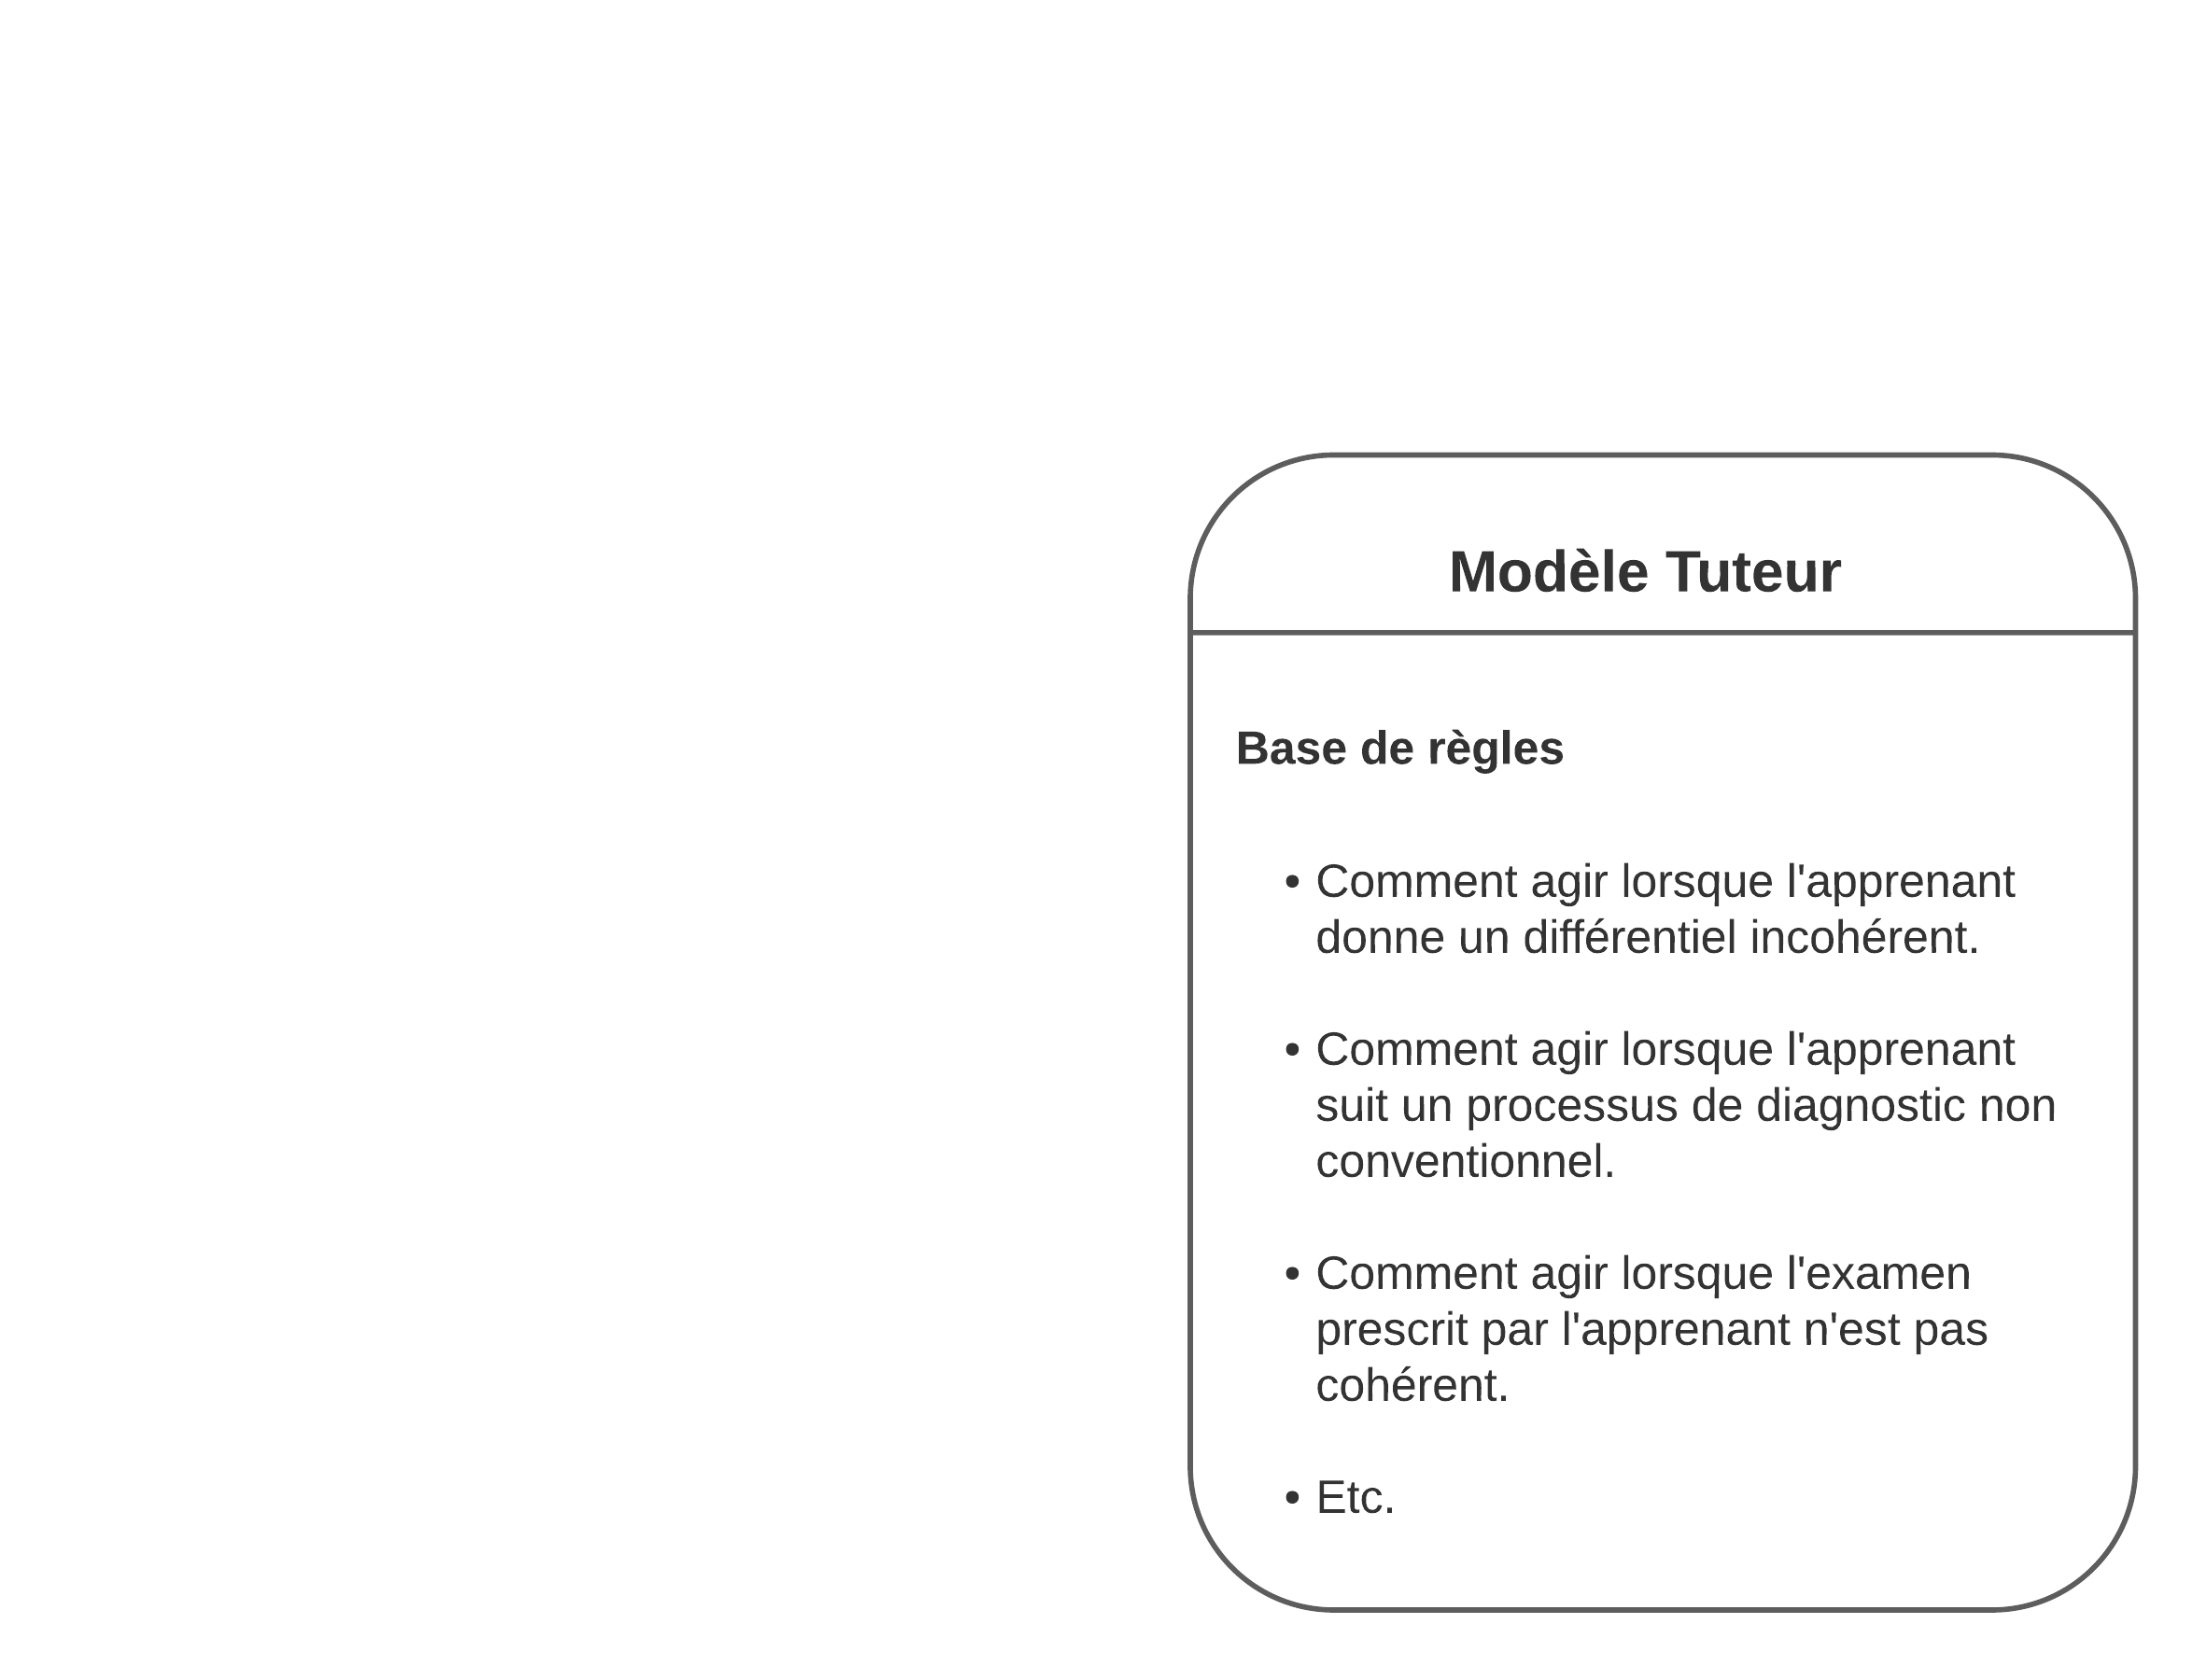
\includegraphics[width=0.75\textwidth]{figures/mod_tuteur.png}
    \captionsetup{justification=centering}
    \caption{Modèle tuteur dans notre STI}
 \label{fig:2}
\end{figure}

\subsubsection{Nos stratégies de feedback}

Nous avons choisi comme catégorie de stratégie le \textit{Knowledge of performance} \textbf{KP} qui fournit à l'apprenant un retour d'informations sommaire après qu'il ai terminé un CAS. Ce feedback contient des informations sur le niveau de performance atteint pour la pose du diagnostic du CAS (par exemple, le pourcentage des bonnes questions) et comme concept élaboré le \textit{Knowledge on how to proceed or, know-how} \textbf{(KH)} \cite{narciss2008feedback} qui doit fournir des informations détaillées sur la connaissance procédurale de la pose de diagnostic du CAS en cours. Il s'agit par exemple des :
\begin{itemize}
    \item Conseils pour la correction des erreurs 
    \item Conseils/explications sur les stratégies spécifiques aux tâches
    \item Conseils/explications sur les étapes du traitement des tâches
    \item Questions d'orientation
    \item Exemples élaborés
\end{itemize}

    \subsection{Modèle Expert}
    Le module expert défini les faits et les règles qui sont valides dans le contexte du diagnostic médical. Il décrit une représentation des connaissances à transmettre à l'apprenant.
    
    Dans ce système, l'objectif est l'enseignement du diagnostic médical. 
    Deux types de connaissances doivent donc être transmises:

    
    \subsubsection{Identification de la maladie}
    L'apprenant doit pouvoir reconnaître à quelle maladie correspond un ensemble de signes et de symptômes manifestés par un patient. L'expert est capable de faire cette correspondance là. Il s'agit alors d'une connaissance descriptive, car c'est un fait qu'un ensemble de symptômes et de signes cliniques sont causés par une maladie particulière.
    
    Pour les connaissances liées à l'identification de la maladie, nous faisons directement la relation entre les signes, symptômes, antécédents et paramètres d'un patient avec la maladie diagnostiquée par l'expert. Pour cela, une base de cas a été mise en place. La base de cas contient des cas réels de patients souffrant d'une maladie qui a pu être diagnostiquée par un expert.
    
    Un cas est caractérisé par:
    \begin{itemize}
        \item Les informations du patient: sexe, âge, condition physique (femme enceinte, etc.)
        \item Les antécédents du patient: maladies, malaises récurrents, etc.
        \item Les paramètres du patient: température, pression sanguine, poids, etc.
        \item Les symptômes du patient
        \item Les signes du patient
    \end{itemize}
    
    
    \subsubsection{Procédure de pose de diagnostic}
    L'expert défini la procédure à suivre, les astuces et les règles à appliquer pour pouvoir établir un bon différentiel le plus rapidement et avec précision. Il s'agit de connaissances procédurales.
    
    A cet effet, nous utilisons un graphe de décision assimilable à un réseau bayésien qui résume les différentes étapes d'un diagnostic médical.
    Les différents noeuds du graphe sont des questions qui peuvent être posée à une étape précise du diagnostic et les liens entre les différents noeuds représentent les réponses possibles qu'un patient peut donner. Les feuilles de l'arbre quant à elles sont les différentes maladies connues de l'expert.
    
    \begin{figure}[H]
        \centering
        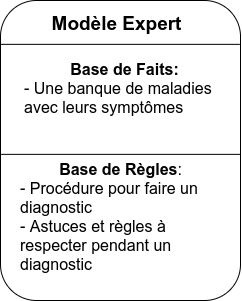
\includegraphics[width=0.35\textwidth]{figures/concept_expert.png}
        \captionsetup{justification=centering}
        \caption{Modèle expert dans notre STI}
        \label{fig:3}
    \end{figure}
    
    \subsubsection{Construction de la procédure de diagnostic chez l'expert}
    Pour construire le graphe de procédure de diagnostic, nous partons de la base des cas. L'idée est de construire un réseau bayésien à partir des différents cas de la base des cas de l'expert.
    Le graphe sera donc une synthèse de la procédure à suivre pour poser un bon diagnostic.
    
    
    \begin{figure}[H]
        \centering
        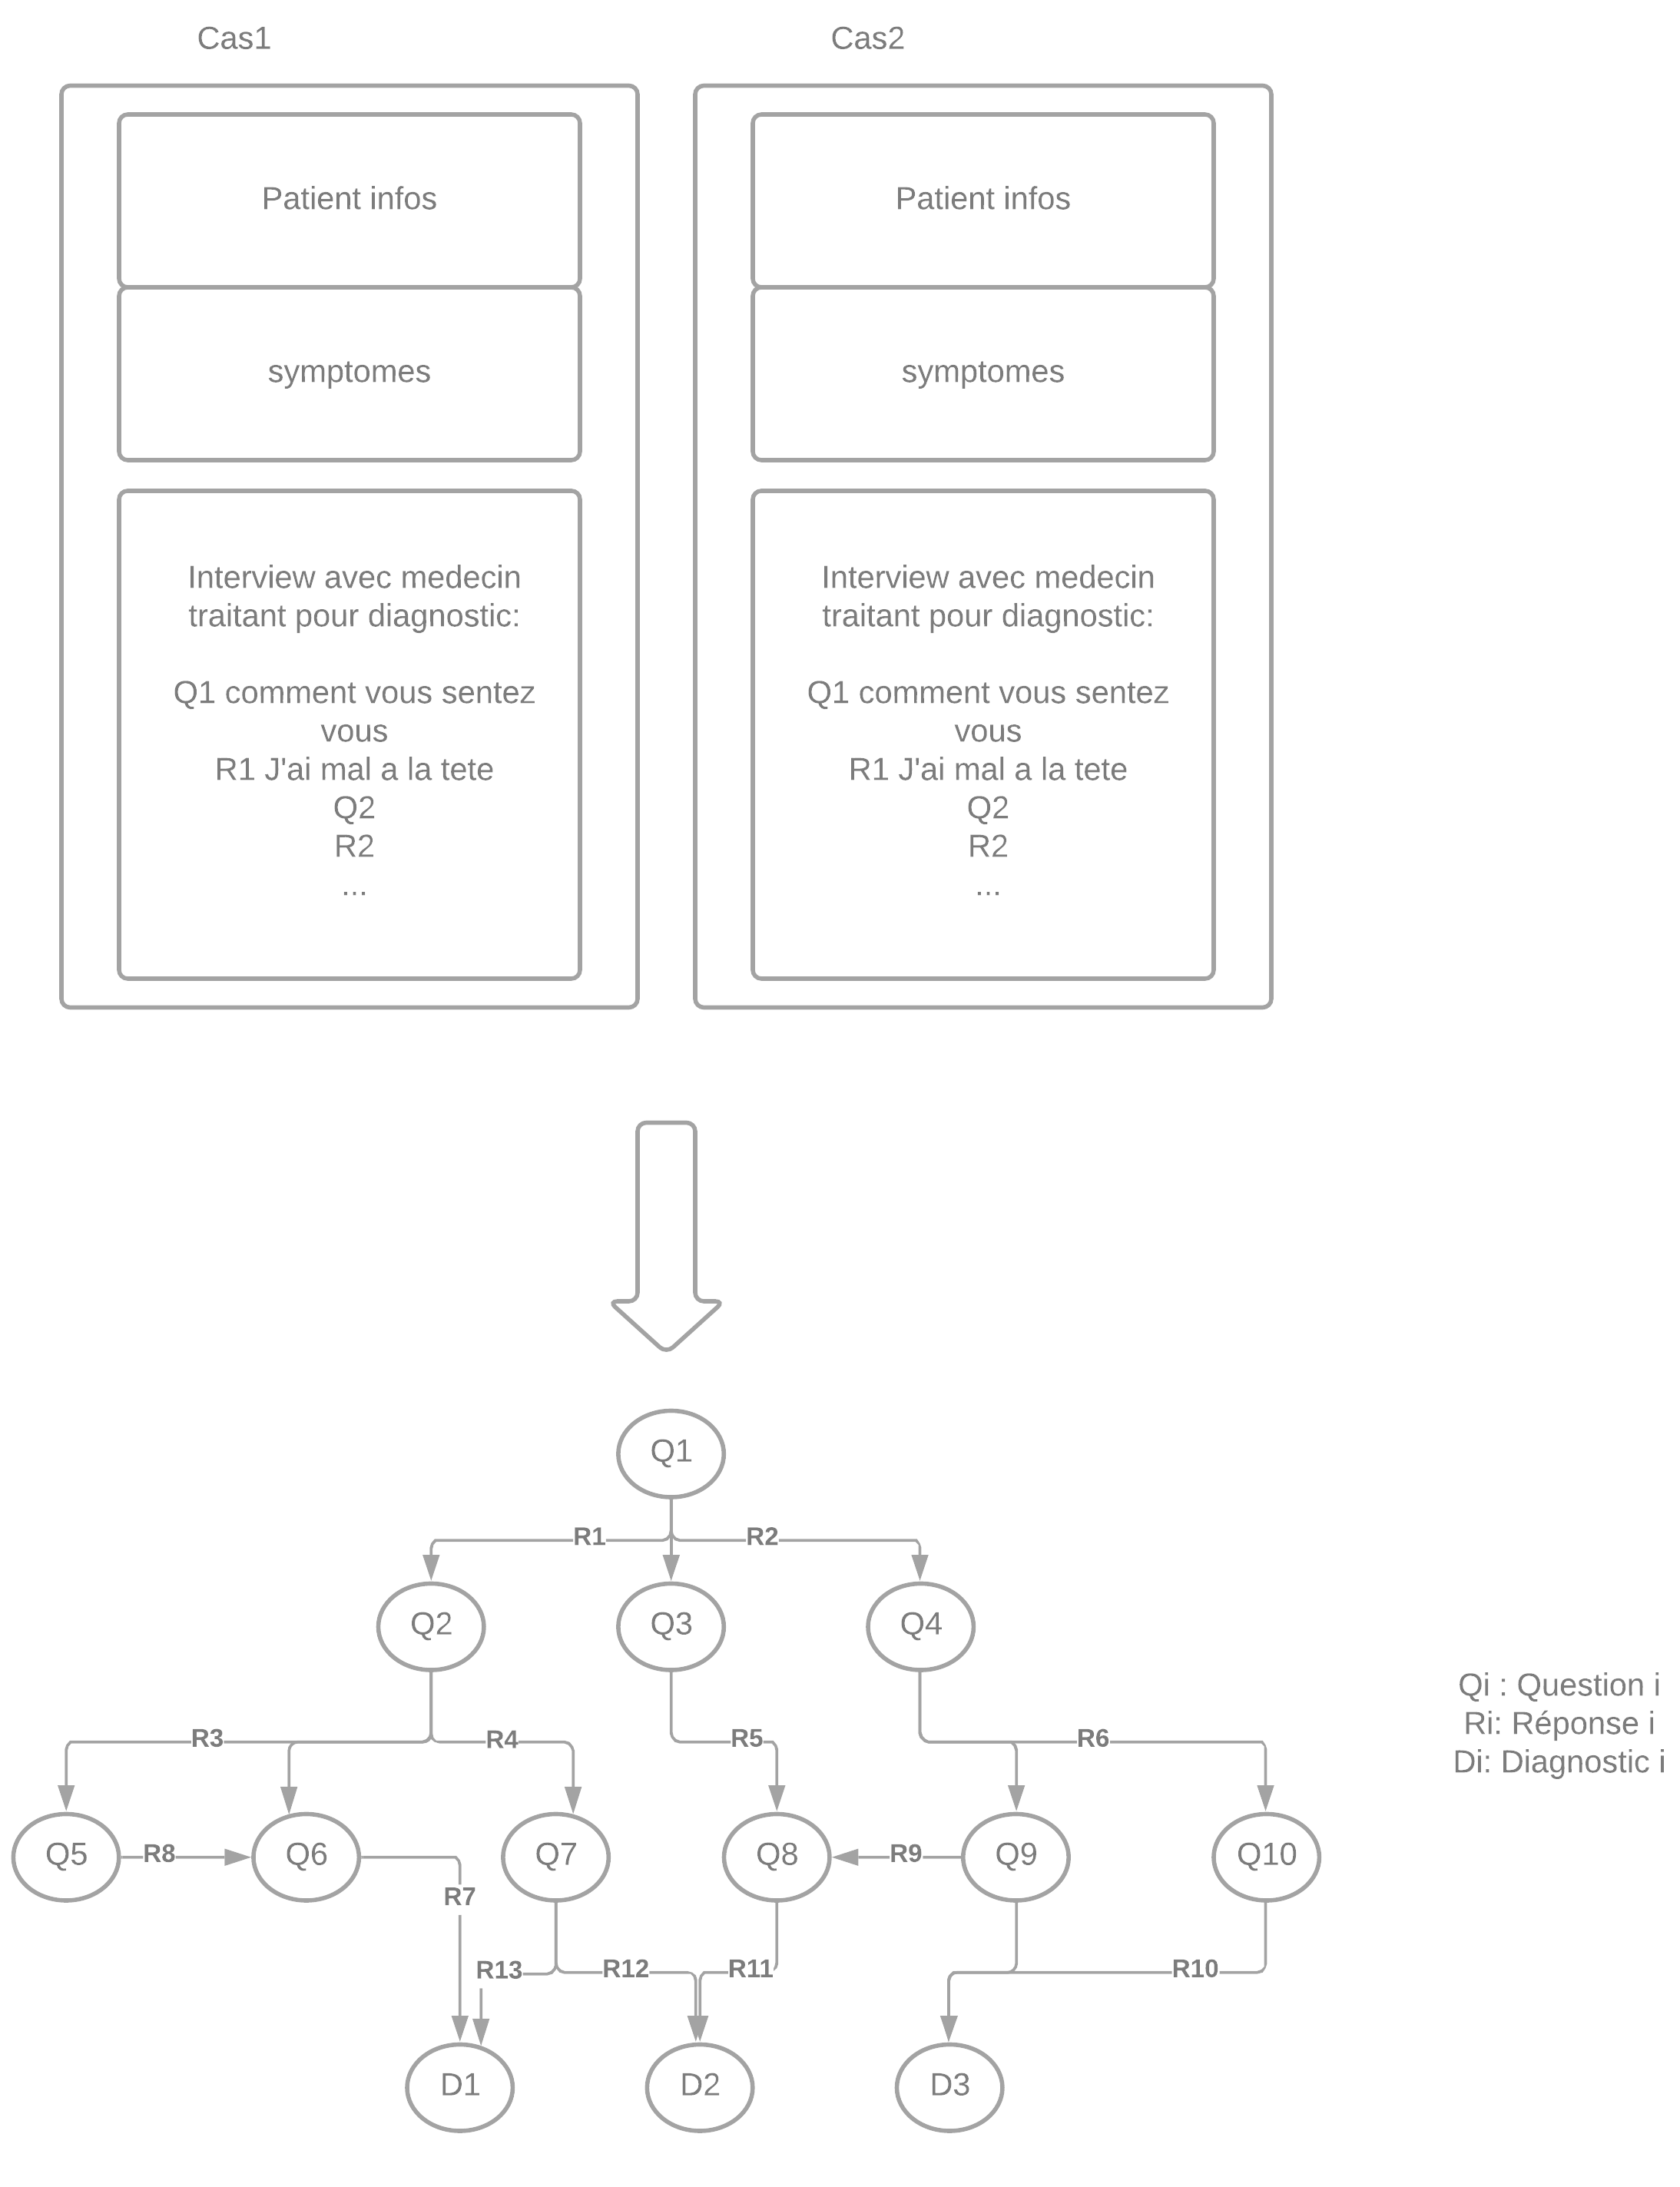
\includegraphics[width=0.75\textwidth]{figures/Trans base cas-reseau bayesien.png}
        \captionsetup{justification=centering}
        \caption{Transformation des cas en réseau bayésien}
        \label{fig:4}
    \end{figure}
    
    \subsection{Patient virtuel}
    Nous considérons dans ce travail que le patient virtuel est un agent émotif et réactif. Il doit être capable de répondre aux questions posées et de simuler une maladie définie par l'expert.
    Comme dans l'architecture de base d'un agent réactif, le patient virtuel possède des actionneurs, des capteurs et un module de traitement.
    
    \subsubsection{Le module capteur}
    Le patient virtuel doit être capable de répondre aux questions posées par l'apprenant. Pour cela, il doit être capable de recevoir et de traiter les questions qui proviennent de l'apprenant via l'interface.
    Le module capteur est donc un module chargé de capturer les questions, qu'elles soient sous forme textuelle ou vocale. En outre, ce module fait du traitement du langage naturel pour extraire de la question l'intention de l'apprenant derrière la question. Les entrées (vocales ou textuelles) sont donc transformées en données représentant les informations d'une question et sont renvoyées vers le module de traitement.
    
    \subsubsection{Le module de traitement}
    Le module de traitement reçoit des données et déclenche les actions à prendre par le patient virtuel. Il reçoit les données du module de capteurs afin d'interroger le module expert pour savoir comment il doit se comporter physiquement et comment il doit répondre aux questions posées par l'apprenant. Il communique donc directement avec le module expert.
    
    \subsubsection{Le module actionneur}
    Le module actionneur permet de définir quel types d'actions le patient virtuel peut effectuer, et comment il doit les effectuer.
    
    Il existe deux types d'actions que le patient virtuel est capable d'effectuer:
    \begin{description}
        \item[Répondre à une question:] Le module permet directement à partir des données renvoyées par le module de traitement de générer un texte ou un message vocal à transmettre à l'apprenant via l'interface. Ce message sert de réponse à une question préalablement posée par ce dernier.
        \item[Manifester les signes physiques d'une maladie:] Ce composant est responsable de simuler les différents tics physique et de donner des méta-informations par rapport aux paramètres a l'apprenant via l'interface.
    \end{description}

    \begin{figure}[H]
        \centering
        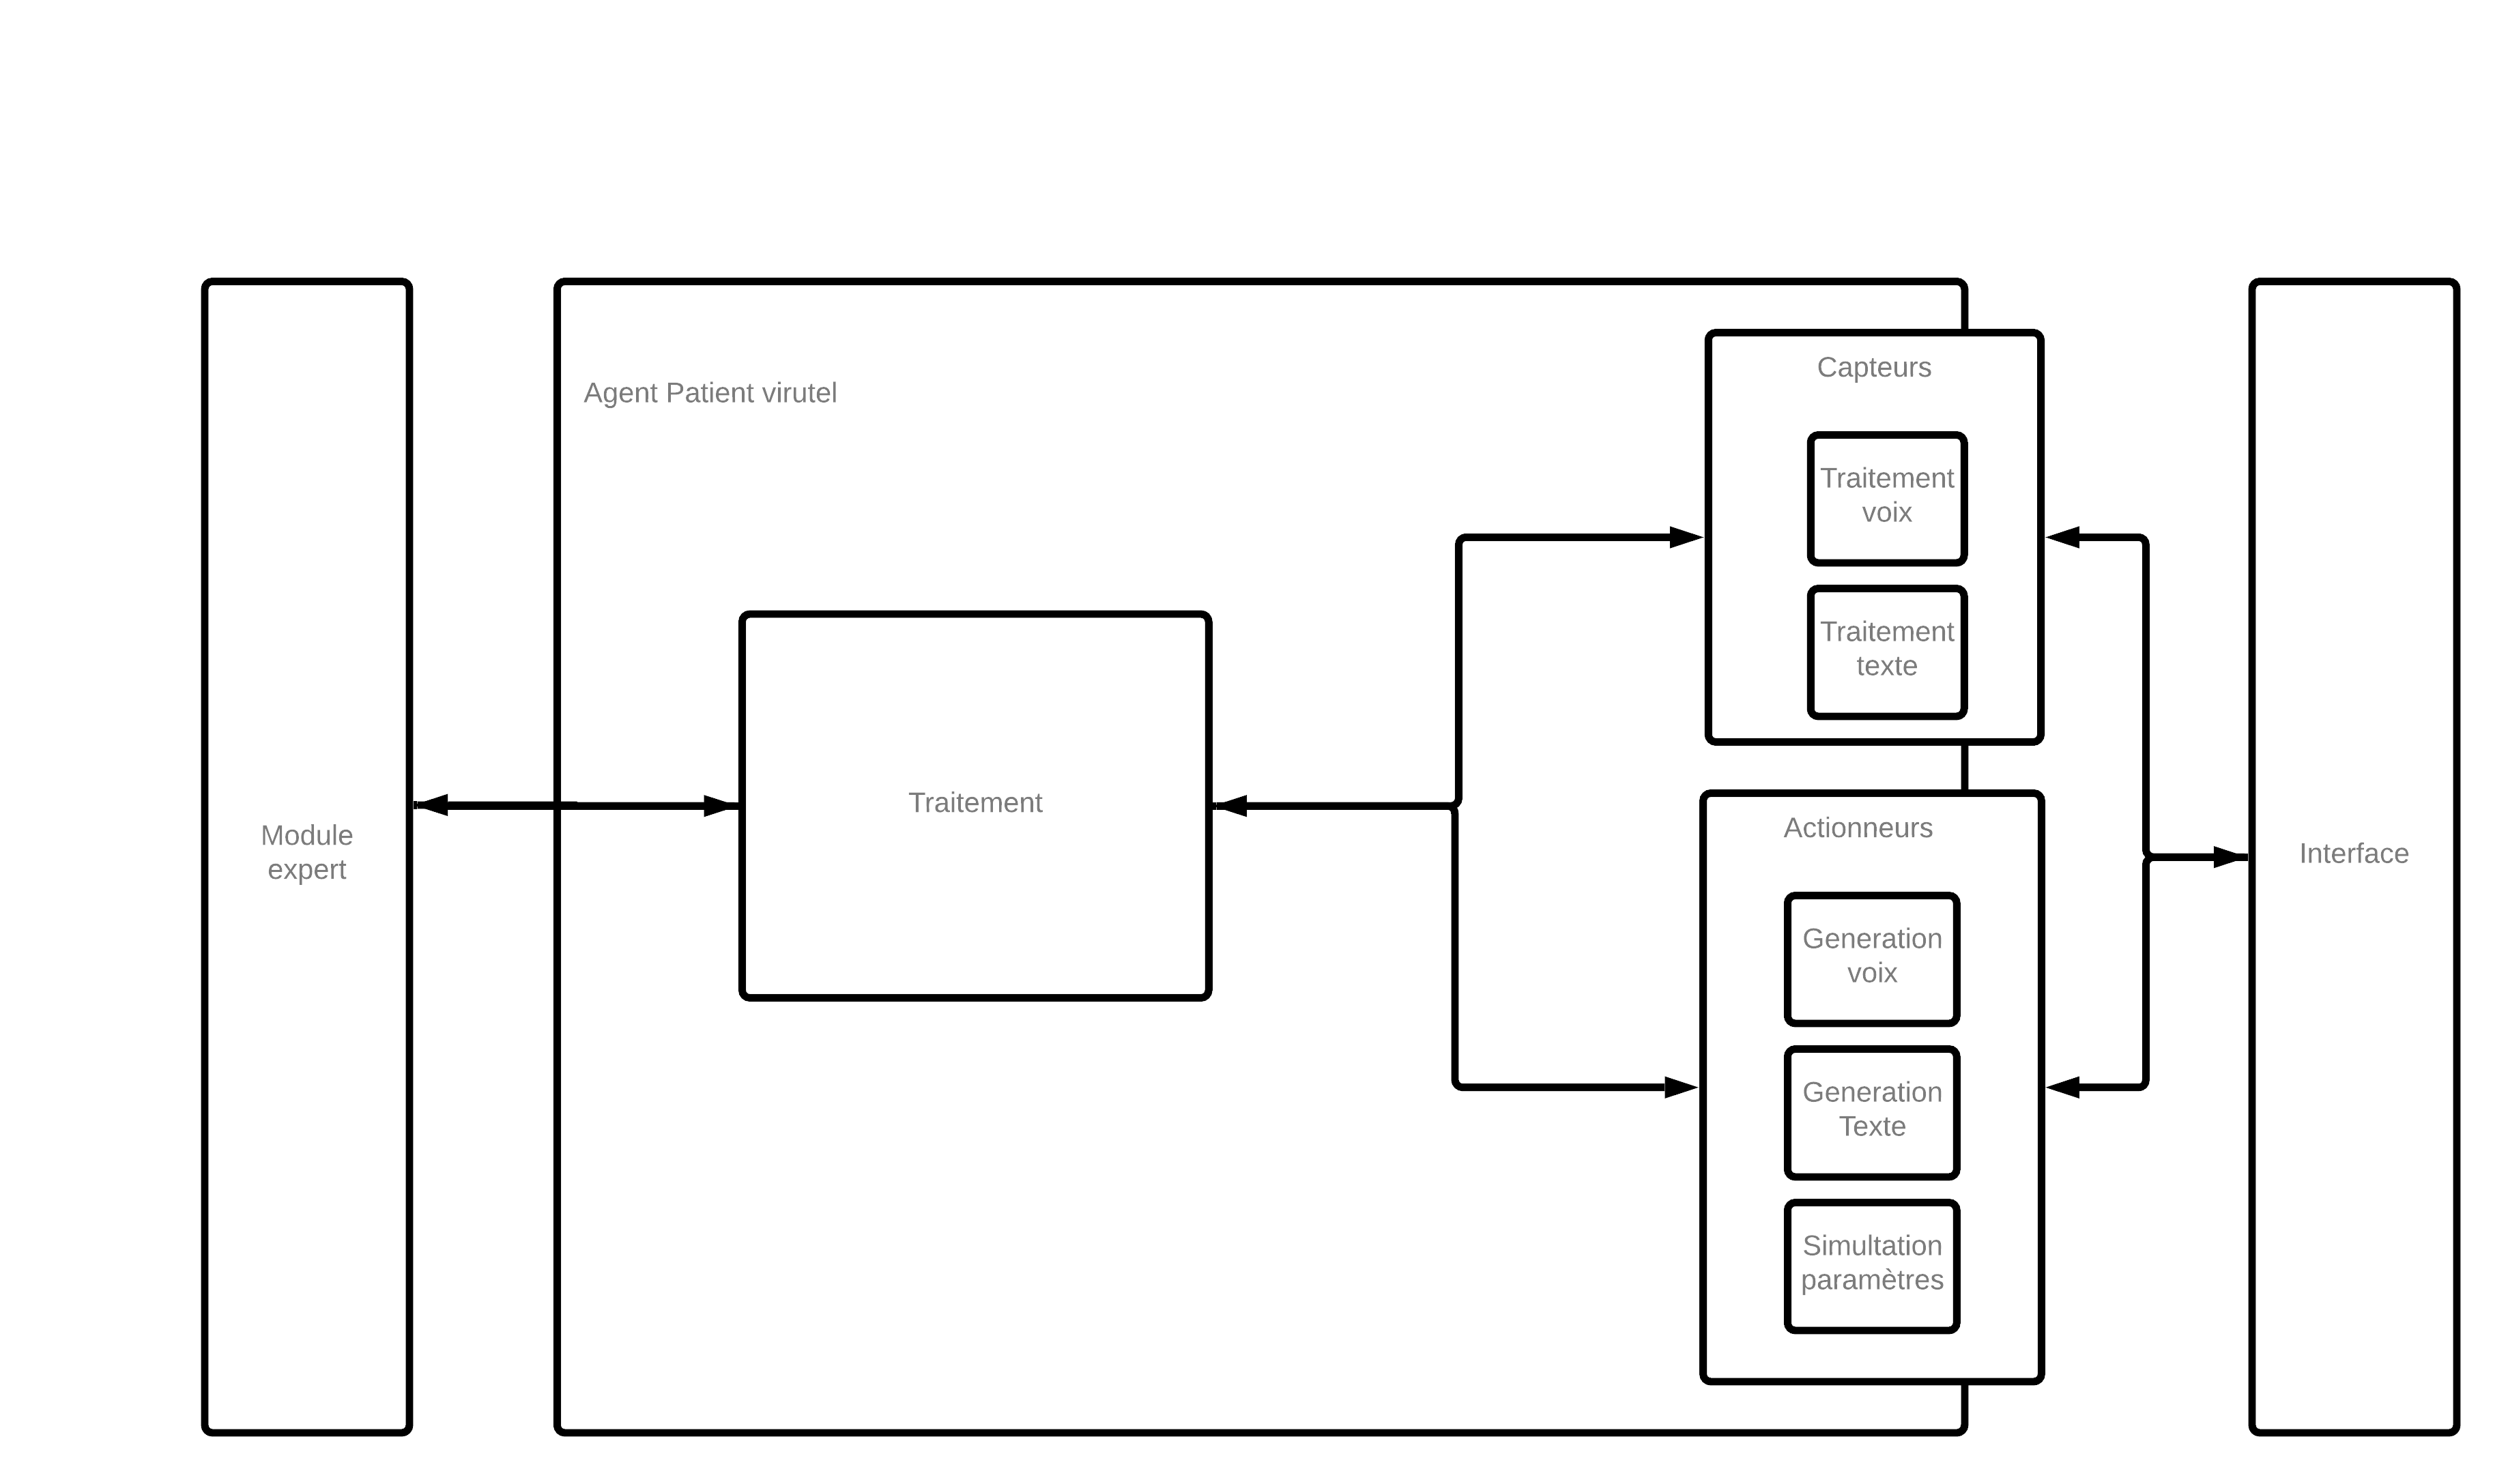
\includegraphics[width=0.75\textwidth]{figures/conc-patient virtuel.png}
        \captionsetup{justification=centering}
        \caption{Module Patient Virtuel}
        \label{fig:5}
    \end{figure}
    
    \subsection{Interface utilisateur}
    Nous utiliserons la méthodologie de la conception centrée sur l'utilisateur. Selon la norme ISO 13407 \cite{iso13407}, cela se fait en 03 étapes:
    \begin{itemize}
        \item Analyse
        \item Conception
        \item Implémentation
    \end{itemize}

    Dans cette section, nous nous intéressons aux parties Analyse et Conception. L'impléméntation sera présenté un peu plus loin dans le document.
    
    \subsubsection{Analyse}
    Il s'agit ici d'identifier la population cible de notre STI, ses caractéristiques, son but et son environnement.
    
    \paragraph{Identification de la population cible} \hfill \\
    Les principaux utilisateurs de notre système ( notre STI) sont :
    \begin{itemize}
        \item des jeunes médecins et
        \item des étudiants médecins
    \end{itemize}
    désirant acquérir le savoir-faire de la pose de diagnostic médical.  À la figure \ref{fig:uml_context}, nous illustration cela dans un diagramme de contexte UML.
    
    \begin{figure}[H]
        \centering
        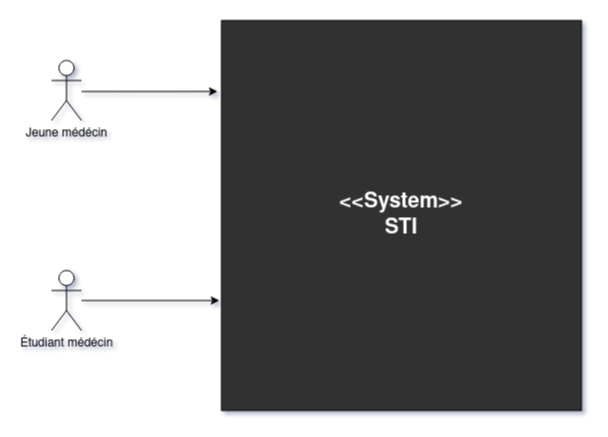
\includegraphics[width=\textwidth]{figures/context.png}
        \captionsetup{justification=centering}
        \caption{Diagramme de Contexte}
        \label{fig:uml_context}
    \end{figure}
    
    \paragraph{Caractéristiques de nos utilisateurs} \hfill \\
    Étant des étudiants médecins ou jeunes médecins, ils seront :
    \begin{itemize}
        \item Relativement jeunes. Entre 16 ans et 35 ans,
        \item des deux sexes , homme et femme, ( je voulais un ratio homme/femme ici ... Mais, ah shit, je ne trouve pas de références)
        \item connaissent les fondamentaux de l'outil informatique et de l'Internet. Par exemple, ils seront ouvrir un site web et le parcourir, reconnaître et remplir des champs de textes, les valider , ....
        
        \item peu expérimentés en ce qui concerne la pose de diagnostic.
    \end{itemize}
    
    \paragraph{But et environnement} \hfill \\
    L'objectif principal de nos utilisateurs est d'apprendre à correctement poser un diagnostic, la méthode et les astuces utilisés par des médecins "experts" ( mieux expérimentés qu'eux). \\
    Nous nous situons dans l'environnement Camerounais. Dans lequel, l'apprentissage assisté par ordinateur est à ses débuts. La forme la plus répandue d'apprentissage assisté par ordinateur sont les cours en ligne : MOOCs (Massive Open Online Courses).En général, ce type d'apprendre est assez rigide. Dans ce sens où les cours , les exercices et les examens sont pré enregistrés de façon peu flexible. Un MOOC ne s'adaptera pas aux spécificités d'un apprenant lambda. Nous nous adressons donc à une population qui n'a "jamais" fait usage des STIs.
    
    \subsubsection{Conception}
    Il s'agit ici de comprendre et spécifier les exigences des utilisateurs, définir les cas d'utilisation.
    À la figure \ref{fig:use_case_user}, nous présentons les différents cas d'utilisation de notre système vus par l'utilisateur et les relations entre eux.
    
    \begin{figure}[H]
        \centering
        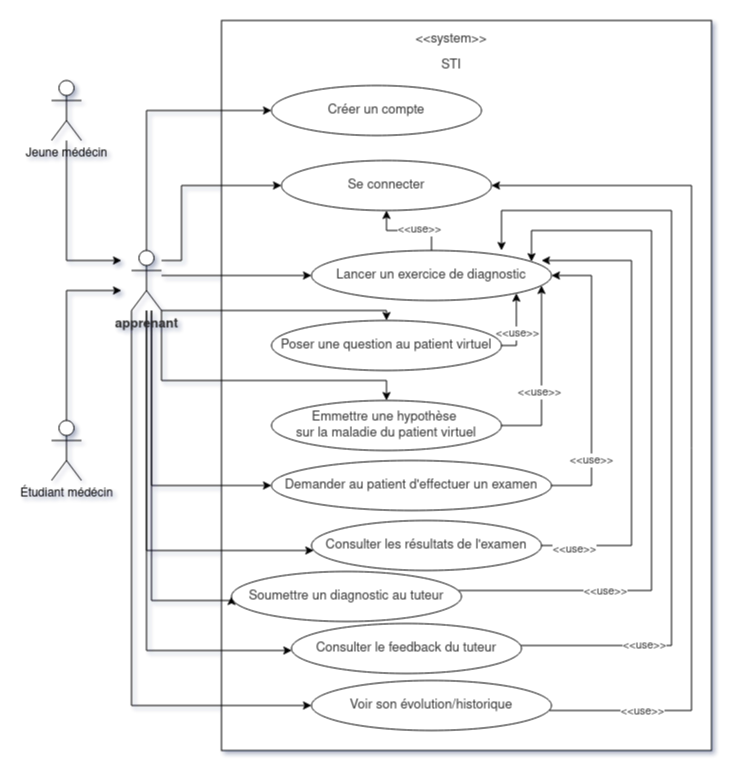
\includegraphics[width=\textwidth]{figures/context-Use case Diagram.png}
        \captionsetup{justification=centering}
        \caption{Diagramme des cas d'utilisation vus par l'utilisateur}
        \label{fig:use_case_user}
    \end{figure}
    \paragraph{Description textuelle de quelques cas d'utilisation.} \hfill \\
    
    \begin{table}[H]
        \centering
        \begin{tabular}{|p{0.3\textwidth}|p{0.7\textwidth}|}
            \hline
            \textbf{Nom} &  Lancer un exercice de diagnostic\\
            \hline
            \textbf{Description}& \\ 
            \hline
            \textbf{Pré conditions}& L'utilisateur doit s'etre connecté à ton compte.\\ 
            \hline
            \textbf{Post condition}& Le patient virtuel est configuré et la partie est lancée.\\ 
            \hline
        \end{tabular}
        
        \captionsetup{justification=centering}
        \caption{Description textuelle de "Lancer un exercice de diagnostic"}
        \label{tab:exercice_use_case}
    \end{table}
    
    \begin{table}[H]
        \centering
        \begin{tabular}{|p{0.3\textwidth}|p{0.7\textwidth}|}
            \hline
            \textbf{Nom} & Demander au patient d'effectuer un examen\\
            \hline
            \textbf{Description}& \\ 
            \hline
            \textbf{Pré conditions}& L'utilisateur doit avoir lancé une partie.\\ 
            \hline
            \textbf{Post condition}& L'examen est effectué et un button permettant d'afficher les résultats de l'examen.\\
            \hline
        \end{tabular}
        
        \captionsetup{justification=centering}
        \caption{Description textuelle de "Demander au patient d'effectuer un examen"}
        \label{tab:examen_use_case}
        
    \end{table}
     \begin{table}[H]
        \centering
        \begin{tabular}{|p{0.3\textwidth}|p{0.7\textwidth}|}
            \hline
            \textbf{Nom} &  Soumettre un diagnostic au tuteur\\
            \hline
            \textbf{Description}& \\ 
            \hline
            \textbf{Pré conditions}& L'utilisateur doit avoir lancé une partie \\ 
            \hline
            \textbf{Post condition}& Le diagnotic posé par l'apprenant est soumi au tuteur et un bouton permettant de charger la la page des résultats et appréciation est affiché.\\
            \hline
        \end{tabular}
        \captionsetup{justification=centering}
        \caption{Description textuelle de "Soumettre un diagnostic au tuteur"}
        \label{tab:diagnostic_use_case}
    \end{table}
    
    \paragraph{Moyens de communication entre l'utilisateur et l'interface.} \hfill \\
    L'utilisateur interagira avec l'interface principalement de deux facons :
    \begin{itemize}
        \item par la vue. \\ Il y aura un certain nombre d'élèments sur son écran sur lesquels il pourra cliquer et voir la réponse à l'écran.
        \item par la voix. \\ La communication avec le patient virtuel se fera aussi par la voix. Similairement aux salons virtuels. Cependant, le système ne peut pas traiter directement de la voix. Nous utiliserons deux modèles de réseaux de neurones, l'un pour la conversion "voice ( speech ) to text" et l'autre pour la conversion "text to speech".
        \begin{itemize}
            \item \textbf{FastSpeech \cite{ren2019fastspeech}} : pour le "text to speech",
            \item \textbf{WaveNet \cite{oord2016wavenet}} : pour le "text to speech".
        \end{itemize}
        Nous illustrons cela à la figure \ref{fig:apprenant_patient_virtuel}.
        \begin{figure}[H]
            \centering
            \hspace*{-0.3in}
            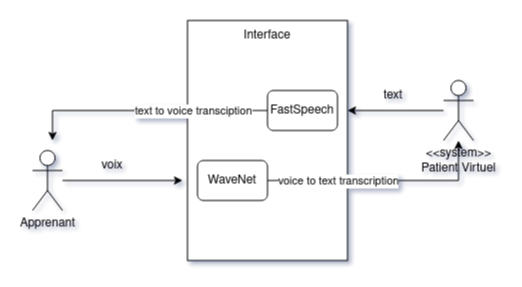
\includegraphics[width=1.1\textwidth]{figures/context-moyens de communication.png}
            \captionsetup{justification=centering}
            \caption{Moyens de communication apprenant-patient virtuel}
            \label{fig:apprenant_patient_virtuel}
        \end{figure}
    \end{itemize}
    
\section{Architecture fonctionnelle}

Après avoir présenté les composantes de notre STI, il est important de comprendre les interactions entre elles ainsi que la manière dont le système les met à contribution pour implémenter les fonctionnalités de notre application.

\subsection{Architecture interne}

Les quatre principaux modules (expert, tuteur, apprenant, interface) et le module du patient virtuel implémentés dans notre système ont été détaillés plus haut dans ce chapitre. La figure \autoref{fig:archi_int} présente un graphique qui illustre les interactions entre les différentes composantes du système.

\begin{figure}[H]

        \centering
        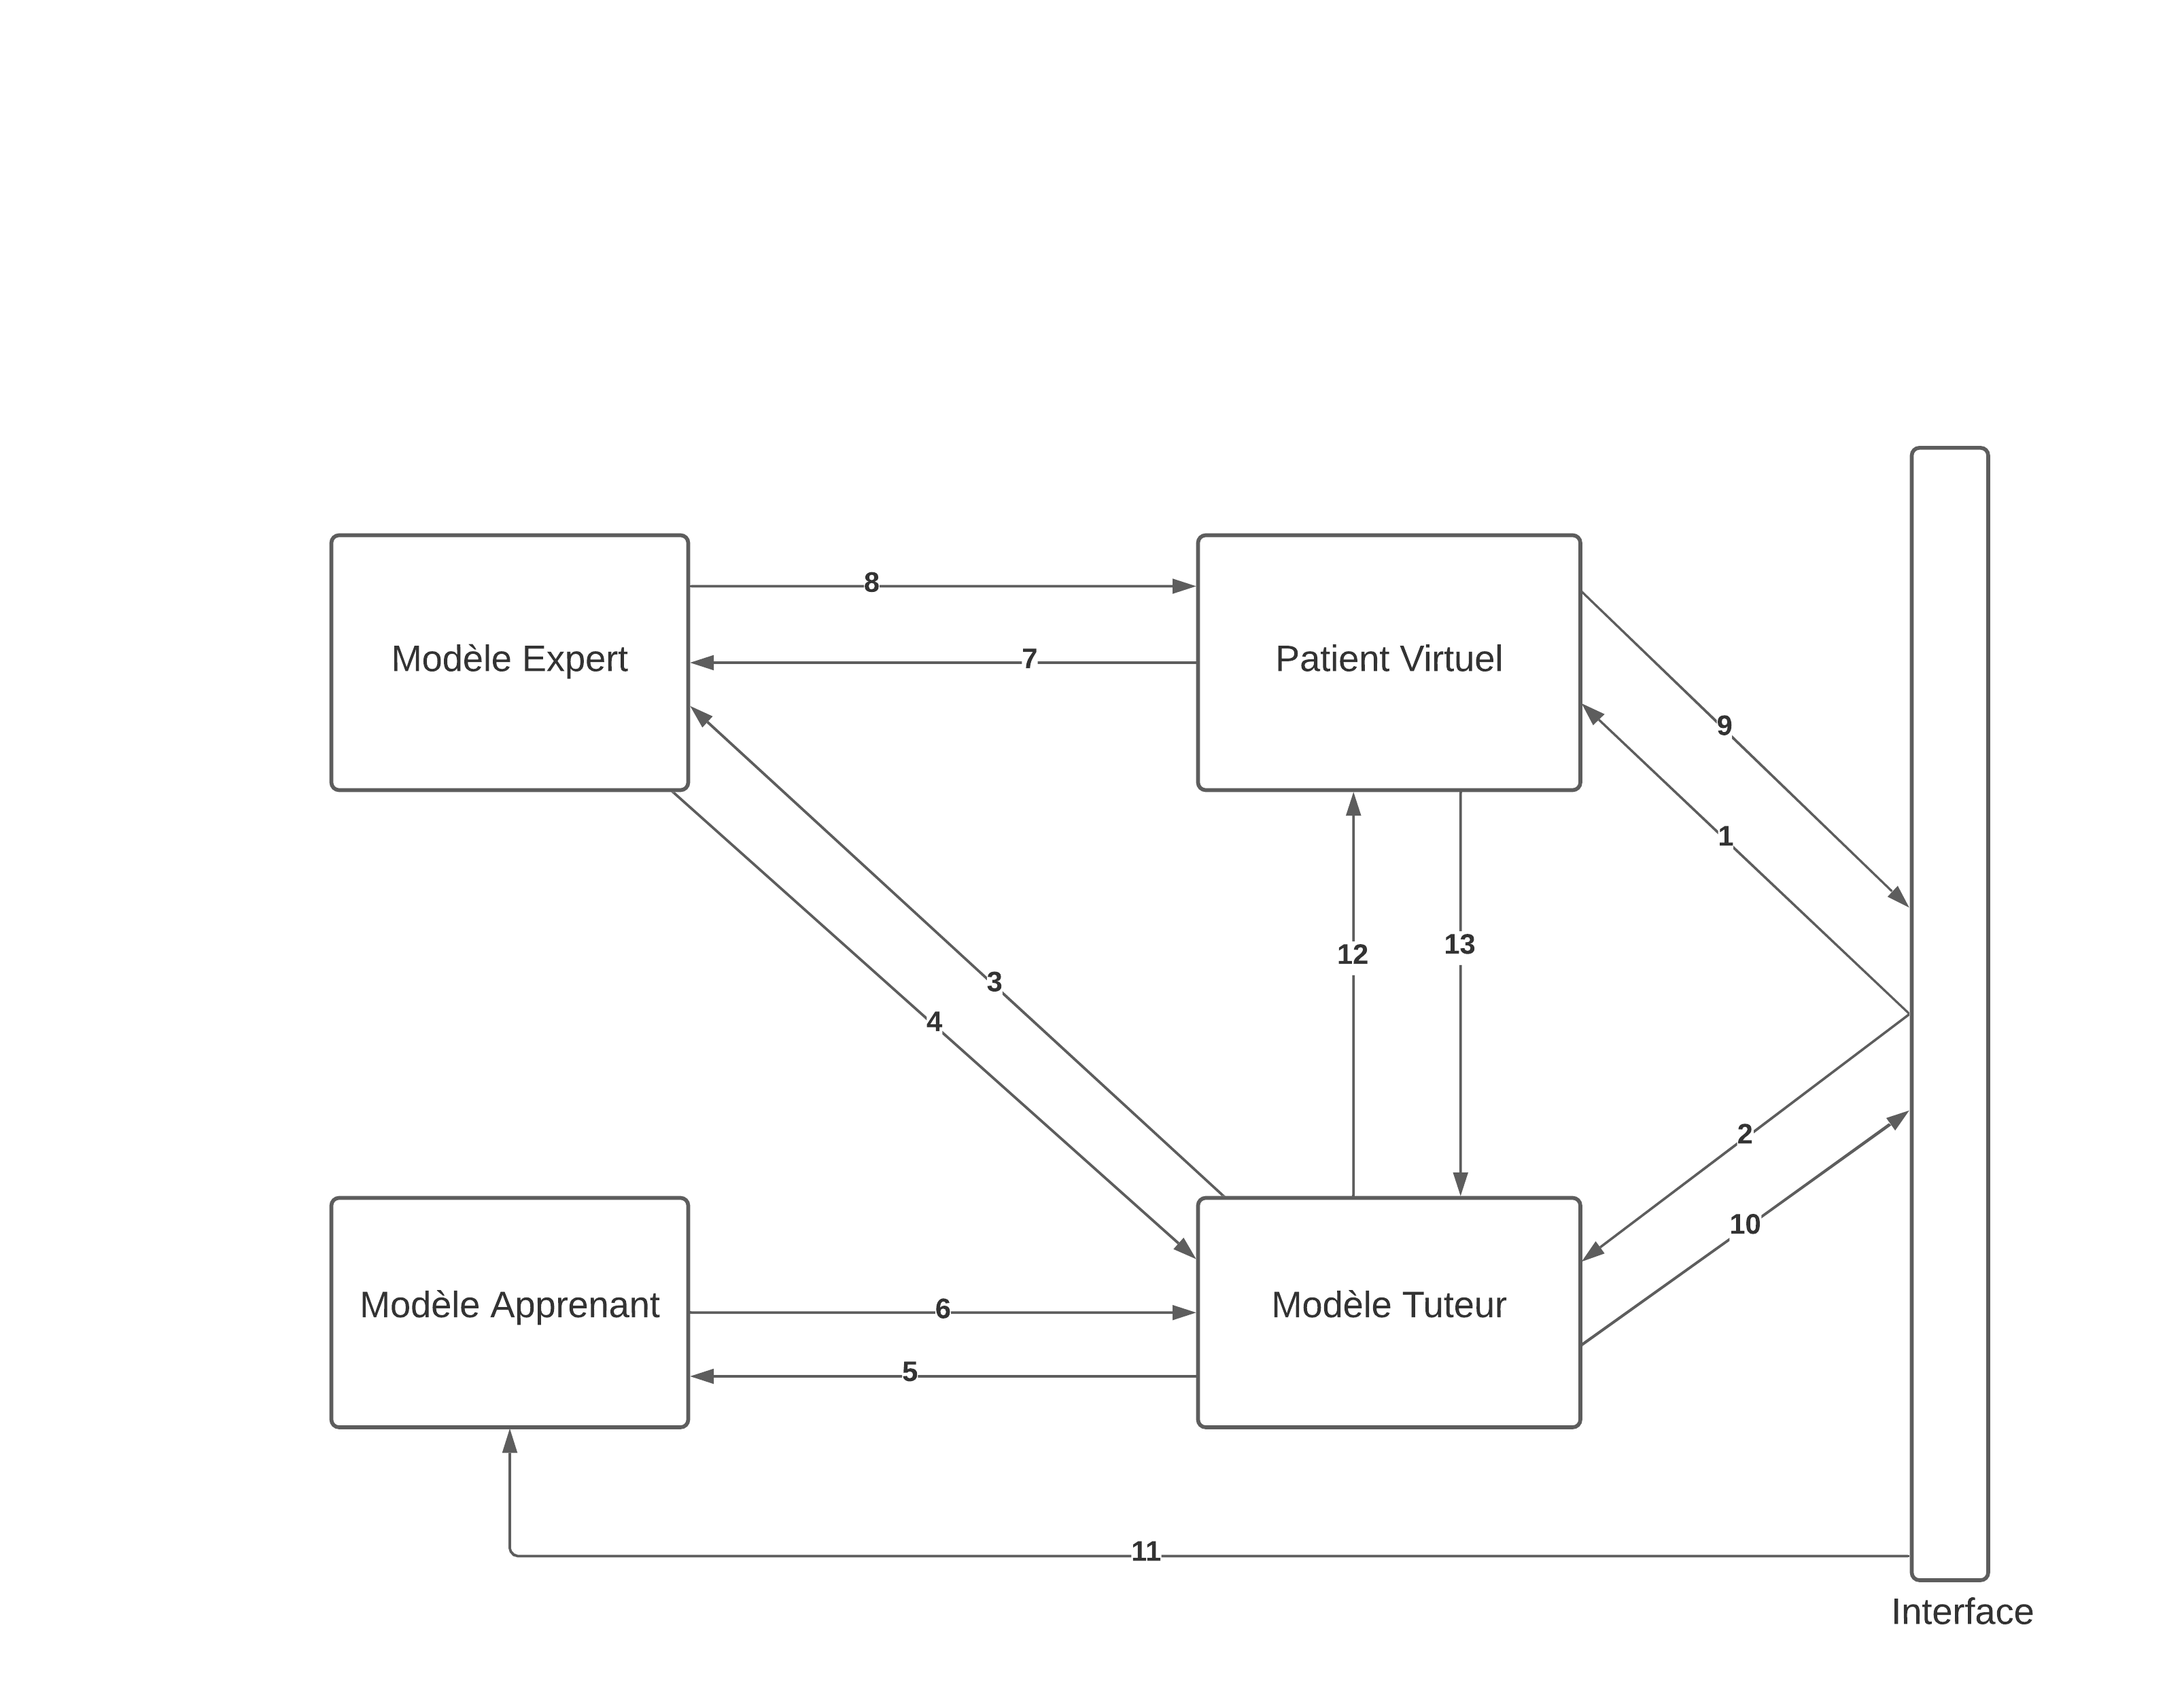
\includegraphics[width=\textwidth]{figures/archi_interne.png}
        \captionsetup{justification=centering}
        \caption{Architecture interne de notre Système}
        \label{fig:archi_int}
\end{figure}


\subsection{Cycle de fonctionnement}
Lorsque l'apprenant démarre l'application, il est invité à entrer les informations de son compte (nom d'utilisateur et mot de passe). Si l'apprenant ne possède pas de compte, il est invité à le créer (noms, niveau scolaire en médecine, année d'expérience, spécialisation, etc ...). Et au tout premier accès, le système lui fait passer un test. Les réponses à ce test serviront à créer le modèle psychométrique qui servira à initialiser le modèle de l'apprenant (\textbf{interaction 1} de la \autoref{fig:archi_int}), permettant au
système d'établir un premier modèle cognitif qui donnera les informations de base sur le suivi personnalisé de l'apprenant.

Après cette première évaluation, l'apprenant médecin peut commencer son apprentissage de la pose de diagnostic médical. Lorsqu'il commence une séance, le modèle Tuteur récupère ses informations contenues dans le modèle apprenant (\textbf{interactions 5} et \textbf{6} de la \autoref{fig:archi_int}) et cherche le \textbf{CAS} le plus approprié pour lui, en fonction de ses informations (spécialité, niveau dans le système, etc ...) en interagissant avec le modèle Expert (\textbf{interactions 3} et \textbf{4} de la \autoref{fig:archi_int}). Une fois le CAS trouvé, la configuration du Patient Virtuel peut commencer, ainsi que de la séance de travail au niveau de l'interface (\textbf{interactions 9,10,12} et \textbf{13} de la \autoref{fig:archi_int}).

Une fois le CAS configuré la séance peut commencer, l'apprenant interagit avec l'interface en posant des questions (par la voix), au patient virtuel, puis l'interface relaie ces questions au Patient Virtuel et au modèle Tuteur (\textbf{interactions 1} et \textbf{2} de la \autoref{fig:archi_int}). Le Patient Virtuel interagit avec le Modèle Expert pour trouver la réponse la plus appropriée du CAS et le transmet à l'interface (\textbf{interactions 7,8} et \textbf{9} de la \autoref{fig:archi_int}). Le modèle Tuteur, dépendamment de ses configurations, conserve le graphe des questions posé et le compare aux graphes procéduraux des questions relatives à tous les CAS du même type en interagissant avec le modèle Expert et le Patient Virtuel (pour les réponses données), ensuite une note est généré avec des feedbacks relatifs à la performance de l'apprenant médecin à l'interface  (\textbf{interactions 3,4,10} et \textbf{12,13} de la \autoref{fig:archi_int}). A la fin le modèle de l'apprenant est mis à jour.

La \autoref{fig:workflow} donne un récapitulatif du workflow du système.



\begin{figure}[H]
        \centering
        \hspace*{-0.6in}
        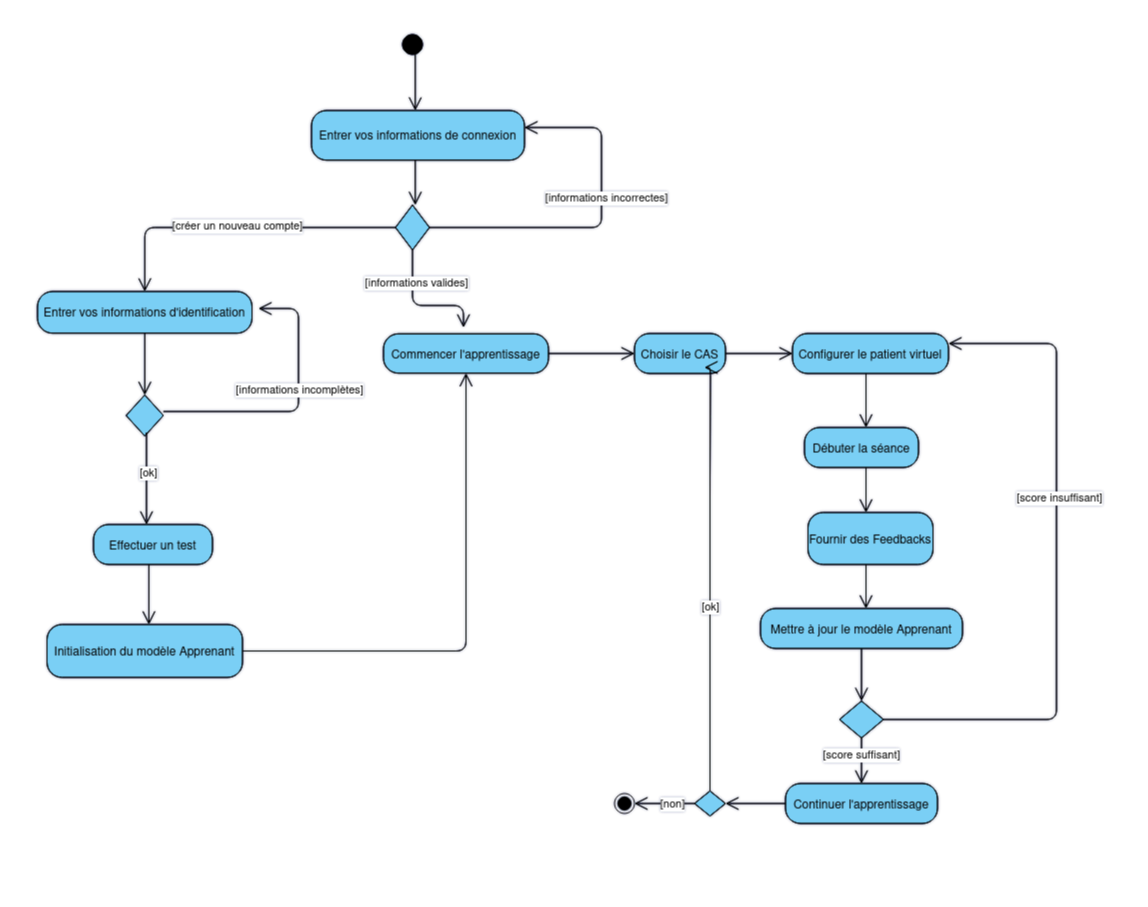
\includegraphics[width=1.2\textwidth]{figures/worflow_STI.png}
        \captionsetup{justification=centering}
        \caption{Workflow du Système}
        \label{fig:workflow}
\end{figure}


% fig de l'archi interne de notre STI
%Example of \autoref{fig:1} reference.

%\begin{figure}
%    \centering
%    \includegraphics[width=0.5\textwidth]{figures/perceptron.png}
%    \caption{Rosenblatt's perceptron.}
%    \label{fig:1}
%\end{figure}
